
\chapter{Feedforward Neural Network Models}

In this chapter, we the greedy tagging system with a feedforward network, which is denoted as Feedforward-History. In the experiments, we show the performance and decoding speed of feedforward models on POS and NER. 

\section{Feedforward-History Model}

Inspired by the greedy parser system by \cite{chen2014fast}, we present a similar greedy transition system for sequence tagging in this thesis. The greedy parser system employs a basic arc-standard system (\citeauthor{nivre2004deterministic}, \citeyear{nivre2004deterministic}), which consists of three types of transitions (LEFT-ARC, RIGHT-ARC, and SHIFT), a stack, and a buffer. While the greedy parser system has three types of actions, the sequence tagging system only needs the SHIFT action which predicts the tag of the current word in the buffer and shifts the word to the stack.  Syntaxnet from Google also uses the same model for POS and dependency parsing and achieves near the state-of-the-art performance on both tasks (\citeauthor{alberti2017syntaxnet}, \citeyear{alberti2017syntaxnet}).

In our greedy tagging system, we use a feedforward network to make decisions on individual words, and we assume that the word to be labeled depends mainly on its neighbor words instead of the whole sentence. Besides the word features, the system also takes into account the lexical composition of the words (spelling features), and the previous tag decisions (previous tag features). Thereby, we represent this architecture as the Feedforward-History model. The way Feedforward-History incorporates word features is the same with the window approach proposed in \cite{collobert2011natural}. The difference between these two models is that Feedforward-History uses spelling features and previous tag features while the model in \cite{collobert2011natural} only uses word features.

\begin{figure}[h]
  \centering
  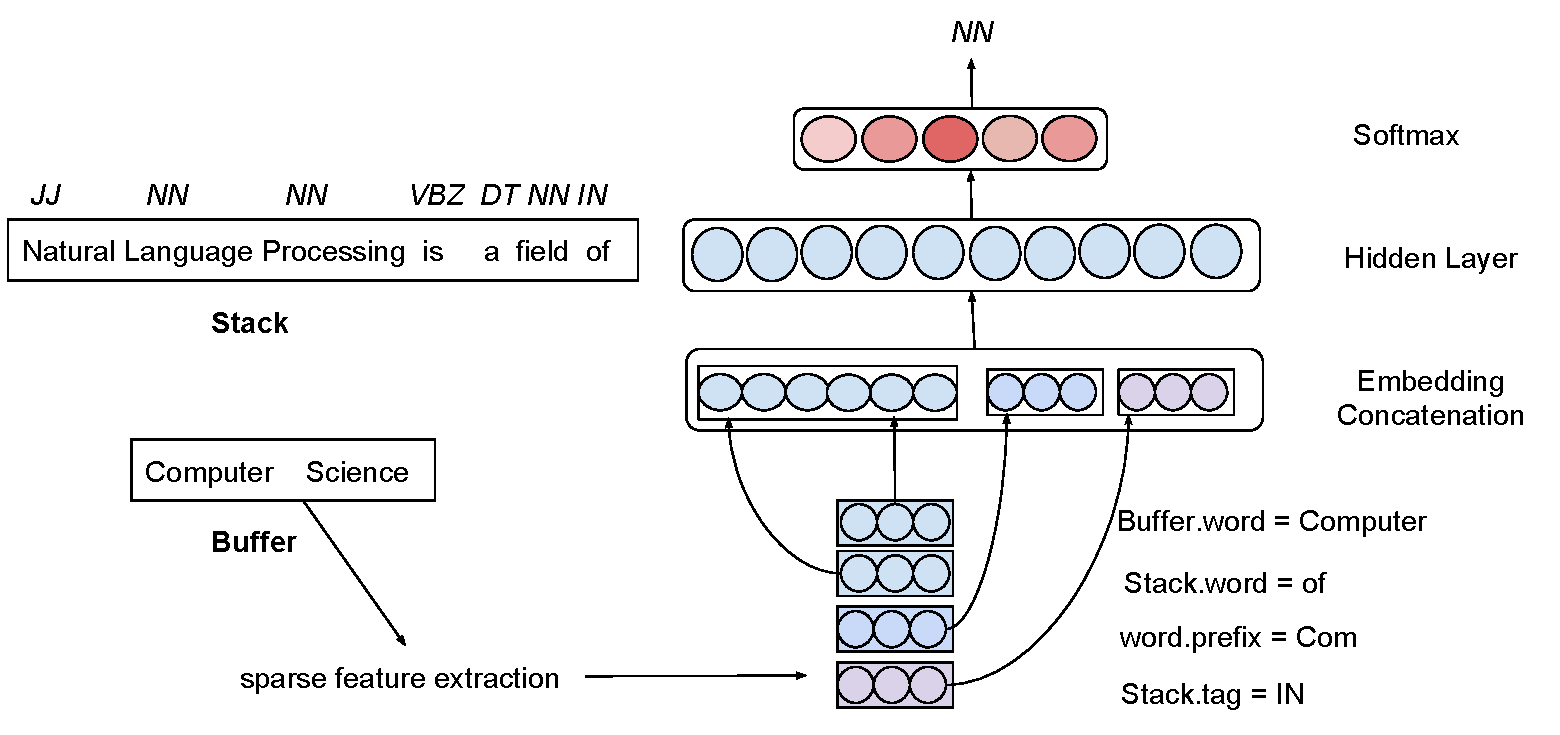
\includegraphics[width=1.0\linewidth]{greedypos.pdf}
 \caption{The architecture of a greedy tagging system using the Feedforward-History model on a POS example.}
  \label{fig:greedypos}
\end{figure}

Figure \ref{fig:greedypos} illustrates the process of how a greedy tagging system uses Feedforward-History to decode a POS example. Since the focused word only depends on its neighbors in this greedy tagging system, we use a fixed size window around the current word to generate features. In order to generate features for the words at the beginning and at the end of the sentence, we add special padding words at the beginning and at the end. To generate dense word features, we convert each word in the input sequence to a $d$-dimensional vector representation $e_{w_{i}}$. Meanwhile, we have a full vocabulary embedding dictionary $E_{w}$. Given a word $w_{i}$, we look up its embedding $e_{w_{i}}$ in $E_{w}$. According to \cite{ratnaparkhi1996maximum}, spelling features of a word can help predict the part-of-speech tag. The examples of spelling features are upper and lower case features, prefix and suffix features, digit features, etc. Each spelling feature of a word is also associated with an embedding vector $e_{s_{i}}$, and it can be looked up from a embedding vector dictionary $E_{s}$. Besides word features and spelling features, we incorporate the previous tag features in this model. Each previous tag decision is represented as $e_{ht_{i}}$ and can be looked up from a tag dictionary represented as $E_{HT}$.

The input layer $X=\left( x_{1},x_{2},\ldots x_{n}\right)$ to the feedforward network is obtained by concatenating the word feature vectors, spelling feature vectors, and previous tag feature vectors. In general, generating a lot of hand-engineered features for sequence tagging is expensive: selecting useful features is an empirical process based on trials and errors, and computing feature vectors requires searching feature strings in huge dictionaries and concatenating them together. We try to use as little hand-engineered features as possible to save the time from feature generation while keeping the model accurate. In our implementation, we extract the following spelling features of each word: whether it starts with a capital letter; whether it has all capital letters; whether it has a mix of letters and digits; whether if has punctuation; and letter prefixes and suffices of length two and three. We also extract 4 previous tags as parts of input features.

While the input layer is the concatenation of the feature vectors of the focused word, the the output layer is a probability distribution over tags. The input unit $x_{i}$ is mapped to a hidden unit $h_{i}$ through the rectifier activation function (\textit{ReLU}) (\citeauthor{nair2010rectified}, \citeyear{nair2010rectified}):

\begin{equation}
\textit{ReLU}\left(x\right) = \textit{Max}\left(0,x\right)
\end{equation}

\begin{equation}
h_{i}=\textit{ReLU}\left( W_{1}^{w}x_{i}^{w}+W_{1}^{s}x_{i}^{s}+W_{1}^{l}x_{i}^{l}+b_{1}\right),
\end{equation}

\noindent
where $x^{w}$ represents the word features, $x^{s}$ represents the spelling features, $x^{l}$ represents previous tag features, $W_{1}$ is the weight parameters in the hidden layer, and $b_{1}$ is the bias of in the hidden layer. The output of the network is a probability distribution over tags, and its dimension is the size of all tags. The tag probability distribution is modeled by a softmax layer:

\begin{equation}
p_{i}=\textit{softmax}\left(W_{2}h_{i}+b_{2}\right),
\end{equation}

\noindent
where $W_{2}$ is the weight parameter in the softmax layer and $b_{2}$ is the bias in the softmax layer. The network is trained by minimizing a negative log likelihood over the training data. Embedding vectors are trained together with weight vectors and bias in the model. We denote all trainable parameters as $\theta$. Given a sequence predictions, $Y=\left( y_{1},y_{2},\ldots y_{n}\right)$,
the score of the output sequence is the sum of the probability of each decision $y_{i}$: 

\begin{equation}
S\left( Y\right) = \sum _{i}^{n}p_{i}\left(y_{i}\right),
\end{equation}

\noindent
and the loss function is:

\begin{equation}
L\left(\theta\right) = -log\left(\sum _{i}^{n}p_{i}\left(y_{i}\right)\right),
\end{equation}

\section{Experiments and Results}

In POS experiments, we train the models using the Penn Treebank training data and development data. Then, we decode the test data using trained models and record the per word accuracy and decoding time. In NER experiments, we train the models using the CoNLL 2003 training data and development data. Then we decode the test data using the trained models, and record the F1 score and decoding time. In Chunking experiments, we train the models using the CoNLL 2000 training data and development data. Then we decode the test data using the trained models, and record the F1 score and decoding time. The speed is measured by the average number of words decoded per second. We are also interested in the robustness of the Feedfoward-History model, so we build a model using a feedforward network with only word features, which serves as the baseline model in our experiments. The tagging system using a feedforward network with only word features is denoted as Feedforward in this thesis.


\begin{table}[h]
\centering
\caption{Hyperparameters used in Feedforward Models}
\label{table:hyperparameters1}
\begin{tabular}{|c|c|}
\hline
Hyperparameters & Values \\ \hline
window size   & 8 \\ \hline
word embedding size & 100 \\ \hline
feedforward layer & 1 \\ \hline
feedforward layer size & 200 \\ \hline
optimizer & Adam \\ \hline
learning rate & 0.01 \\ \hline
batch size & 32 \\ \hline
\end{tabular}
\end{table}

\begin{table}[h]
\centering
\caption{Performance of Feedforward Models on POS}
\label{table:ff-table1}
\begin{tabular}{|c|c|c|}
\hline
Model          & Accuracy       & Error Reduction (words)      \\ \hline
Feedforward    & 95.89          & $-$     \\ \hline
Feedforward-History & 97.28 (+1.39)    & 788 \\ \hline
BiLSTM-CRF & 97.34 (+1.45) & 822 \\ \hline
\end{tabular}
\bigskip
\caption{Performance of Feedforward Models on NER CoNLL 2003}
\label{table:ff-table2}
\begin{tabular}{|c|c|c|c|}
\hline
Model          & Precision   & Recall   & F1 \\ \hline
Feedforward    & 82.99       & 83.59    & 83.29 \\ \hline
Feedforward-History & 87.68  & 87.27    & 87.47 (+4.18) \\ \hline
BiLSTM-CRF & 89.93 & 90.16 & 90.05 (+6.76) \\ \hline
\end{tabular}
\bigskip
\caption{Performance of Feedforward Models on Chunking}
\label{table:ff-table3}
\begin{tabular}{|c|c|c|c|}
\hline
Model          & Precision   & Recall   & F1 \\ \hline
Feedforward    & 89.35       & 91.55    & 90.43 \\ \hline
Feedforward-History & 92.52  & 92.69    & 92.61 (+2.18) \\ \hline
BiLSTM-CRF & 93.91 & 93.81 & 93.86 (+3.43) \\ \hline
\end{tabular}
\end{table}

\begin{table}[h]
\centering
\caption{Feedforward Models Decoding Speed (words/sec)}
\label{table:ff-tabel4}
\begin{tabular}{|c|c|c|c|}
\hline
Model       & POS & NER (CoNLL 2003) & Chunking     \\ \hline
Feedforward    & 30967     & 26819  &16920  \\ \hline
Feedforward-History & 19474 (-1.59$\times$) & 17609 (-1.52$\times$) & 10067 (-1.68$\times$)  \\ \hline
BiLSTM-CRF & 9009 (-3.43$\times$) & 10100 (-2.65$\times$) & 5390 (-3.14$\times$)\\ \hline
\end{tabular}
\end{table}

The hardware specifications are listed in Table \ref{table:hardware}. In NER experiments, because of the small amount of training data, we use GloVE pretrained word embedding where each word corresponds to a 100-dimensional embedding vector. We use the hyperparameters defined in Syntaxnet (\citeauthor{alberti2017syntaxnet}, \citeyear{alberti2017syntaxnet}), which contains a greedy POS tagging system shown to achieve near the state-of-the-art performance. Specifically we use Adam (\citeauthor{kingma2014adam}, \citeyear{kingma2014adam}) for stochastic optimization, and set the learning rate to be 0.01. We use 1 hidden layer and set the hidden layer size to be 200. We have a batch implementation which can process multiple sentences at the same time, and we set the batch size to be 32 in the experiments. Table \ref{table:hyperparameters1} shows the hyperparameters. We initialize all the weight parameters using Xavier initialization (\citeauthor{glorot2011domain}, \citeyear{glorot2011domain}). The experiments specification is shown in Table \ref{table:hardware}.


Table \ref{table:ff-table1} presents the POS results achieved by greedy feedforward models and BiLSTM-CRF. Table \ref{table:ff-table2} presents the final benchmark results including Precision, Recall, and F1 score of feedforward models on NER. Table \ref{table:ff-table3} presents the performance of the models on Chunking. In all three sequence tagging tasks, BiLSTM-CRF outperforms Feedforward-History. BiLSTM-CRF improves the NER performance the most because of the dependencies among output tags. Table \ref{table:ff-tabel4} shows the decoding speed of Feedforward and \ffa. \ffa{} has faster decoding speed then BiLSTM-CRF on all three sequence tagging tasks.



